\section{Introduction}
The transportation sector is dominantly powered by petroleum-based fuels \cite{davis2009transportation}. In the US, it is responsible for 36\% of energy-related carbon dioxide emissions \cite{useia} and 50,000 premature deaths per year associated with particulate matter and ozone emissions \cite{caiazzo2013air}. 
Natural gas and hydrogen (H$_2$) are alternative transportation fuels that emit fewer/less pollutants 
than petroleum-based fuels, and thus their widespread adoption could mitigate climate change 
\cite{mcglade2015geographical} and improve air quality for human health. Further, as the finite global 
petroleum resources are declining rapidly \cite{sorrell2010global}, the development of technologies for the widespread
adoption of sustainable transportation fuels, such as hydrogen, is critical.

Natural gas, mostly methane, is considered a transition (to a renewable and clean) fuel because 
it emits 25\% less carbon dioxide \cite{eia2013much} and less toxic 
byproducts \cite{wang2000full} upon combustion per unit energy produced compared to gasoline. From an 
economic standpoint, the supply of natural gas in the US is increasing as a result of hydraulic 
fracturing and horizontal drilling techniques \cite{usnatgassupply}. A positive environmental outlook 
for natural gas, however, is predicated on mitigating fugitive emissions (methane is itself a potent 
greenhouse gas) \cite{alvarez2012greater} and groundwater contamination \cite{osborn2011methane}
from hydraulic fracturing.

Hydrogen (H$_2$) is the ultimate transportation fuel because it emits only water when it electrochemically reacts with oxygen in a fuel cell to produce electricity and power a vehicle.
% Moreover, elemental hydrogen is very abundant, though bonded with oxygen (in water) or carbon (in hydrocarbons); H$_2$ does not occur naturally in abundant quantities.
Currently, hydrogen (H$_2$) is primarily produced by steam reforming of natural gas followed by the
water-gas shift reaction, which emits carbon dioxide \cite{crabtree2004hydrogen}. Notably, the 
environmental allure of hydrogen is predicated on its production via a renewable means, e.g.\ splitting
water using wind-generated electricity.

% \jordan{I got the values from wikipedia but the citation that wikipedia gave didn't link to the correct paper? Article is Energy Density.
% THIS PAPER says H2 at 700 bar is 4.7 MJ/L: Review on processing of metal–organic framework (MOF) materials towards system integration for hydrogen storage
% }
At ambient conditions, both methane
%(0.036 MJ/L)
and hydrogen gas
%(0.01 MJ/L)
possess a very low volumetric energy density compared to (liquid) gasoline.
%(34.2 MJ/L)
Consequently, under storage space constraints in passenger vehicles, natural gas and hydrogen must be densified for onboard storage to achieve a reasonable driving range on a ``full'' tank of fuel. Traditional densification approaches are liquefaction (cryogenic storage near atmospheric pressure)
% (at 1 atm, liquid CH$_4$ at 111~K to achieve 22.2 MJ/L~\cite{makal2012methane}, liquid H$_2$ at 20 K to achieve 8~MJ/L \cite{suh2011hydrogen})
or compression to high pressures (room temperature storage).
% (200 bar for CH$_4$ to achieve 9.2 MJ/L \cite{makal2012methane} and 700 bar for H$_2$ to achieve 4.5-5.3 MJ/L~\cite{unknown}).
Both approaches require expensive infrastructure at refilling stations and significant energy input; e.g., liquefaction of hydrogen consumes at least 30\% of its energy content~\cite{bossel2003energy}. Moreover, high-pressure storage tanks are heavy, thick-walled, and non-conformable, while cryogenic storage tanks are bulky, expensive, and afflicted by boil-off losses~\cite{hasan2009minimizing}.
% \jordan{
% Both forms of densification suffer several drawbacks varying from safety issues,  excessively expensive, boil-off~\cite{hasan2009minimizing}, and extensive refilling infrastructure~\cite{bossel2003energy}. 
% }
% % Jordan: I commented this out! % Cory: I shorted it. I think it's important.

A promising approach to densify natural gas~\cite{makal2012methane,mason2014evaluating} and hydrogen~\cite{suh2011hydrogen,garcia2018benchmark} for vehicular storage is through physical adsorption in nanoporous materials at room temperature~\cite{schoedel2016role}. The internal surfaces of porous materials attract gas molecules through van der Waals, electrostatic, etc. interactions to achieve a higher adsorbed gas density than the bulk gas at the same temperature and pressure, allowing for room temperature and lower-pressure storage and alleviating many drawbacks of high-pressure storage.
% This would thereby reduce the cost of infrastructure at refilling stations, allow thinner-walled and therefore cheaper and lighter pressure vessels, reduce the energy requirements for gas densification, and alleviate safety concerns with high pressure storage. 

%As most homes in the US are connected to a natural gas pipeline \addcite, adsorbed natural gas fuel tanks could permit at-home fueling.

% Jordan: I commented this out!
% Cory: I think I agree that this paragraph is not necessary, thanks.
% Current research is towards synthesizing a nanoporous material that can maximally densify natural gas/hydrogen whilst satisfying cost and stability constraints. So far, metal-organic frameworks (MOFs) \cite{furukawa2013chemistry} have demonstrated the highest internal surface areas ($>$7000 m$^2$/g \cite{farha2012metal}) and absorptive capacities for hydrogen \cite{suh2011hydrogen,garcia2018benchmark} and methane \cite{makal2012methane,mason2014evaluating}. Importantly, MOFs are highly adjustable materials synthesized by combining organic molecules (struts) and metal clusters (nodes) that
% % I cut [often] here, since I'm not sure what the exception is and I don't think it's relevant.
% coordinate to form a three-dimensional, porous framework \cite{furukawa2013chemistry}. This modular synthesis enables one to fine-tune the MOF chemistry to arrive at an optimal material for methane or hydrogen storage and delivery \cite{schoedel2016role}. See Fig.~\ref{fig:example_MOF} for the crystal structure of a canonical MOF, CuBTC \cite{chui1999chemically}.

For a vehicle employing a porous material to store natural gas or hydrogen, the (volumetric) \emph{deliverable capacity} of the gas is the primary thermodynamic property of the material that determines the driving range~\cite{mason2014evaluating}. The adsorbed gas storage tank delivers the gaseous fuel to the engine via an (assumed) isothermal pressure swing~\cite{sircar2002pressure}. The deliverable capacity (see Fig.~\ref{fig:delcap}) is the density of the gas in the material at the storage pressure $\pfull$ minus the residual gas that remains adsorbed at the lowest pressure $\pempty$ such that sufficient flow is maintained to feed the engine.
For commercial feasibility, the US Department of Energy (DOE) has set deliverable capacity targets for both adsorbed methane and hydrogen storage and delivery for vehicles. For methane, the Advanced Research Projects Agency--Energy (ARPA-E) set a deliverable capacity target of 315\ L STP CH$_4$ per L of adsorbent at 298 K using a 65\ bar to 5.8\ bar pressure swing~\cite{simon2015materials}. For hydrogen, the DOE set a series of progressive targets at five year intervals, with the ultimate target of 0.05 kg H$_2$/L~\cite{h2targetsDOE} using a 100\ bar to 5\ bar pressure swing at a minimum of -40 $^\circ$C~\cite{allendorf2018assessment}. Thus far, despite the emergence of highly tunable materials with enormous surface areas, such as metal-organic frameworks~\cite{furukawa2013chemistry}, no porous material has met these deliverable capacity targets. 

\begin{figure}
    \centering
    \subfloat[][]{
        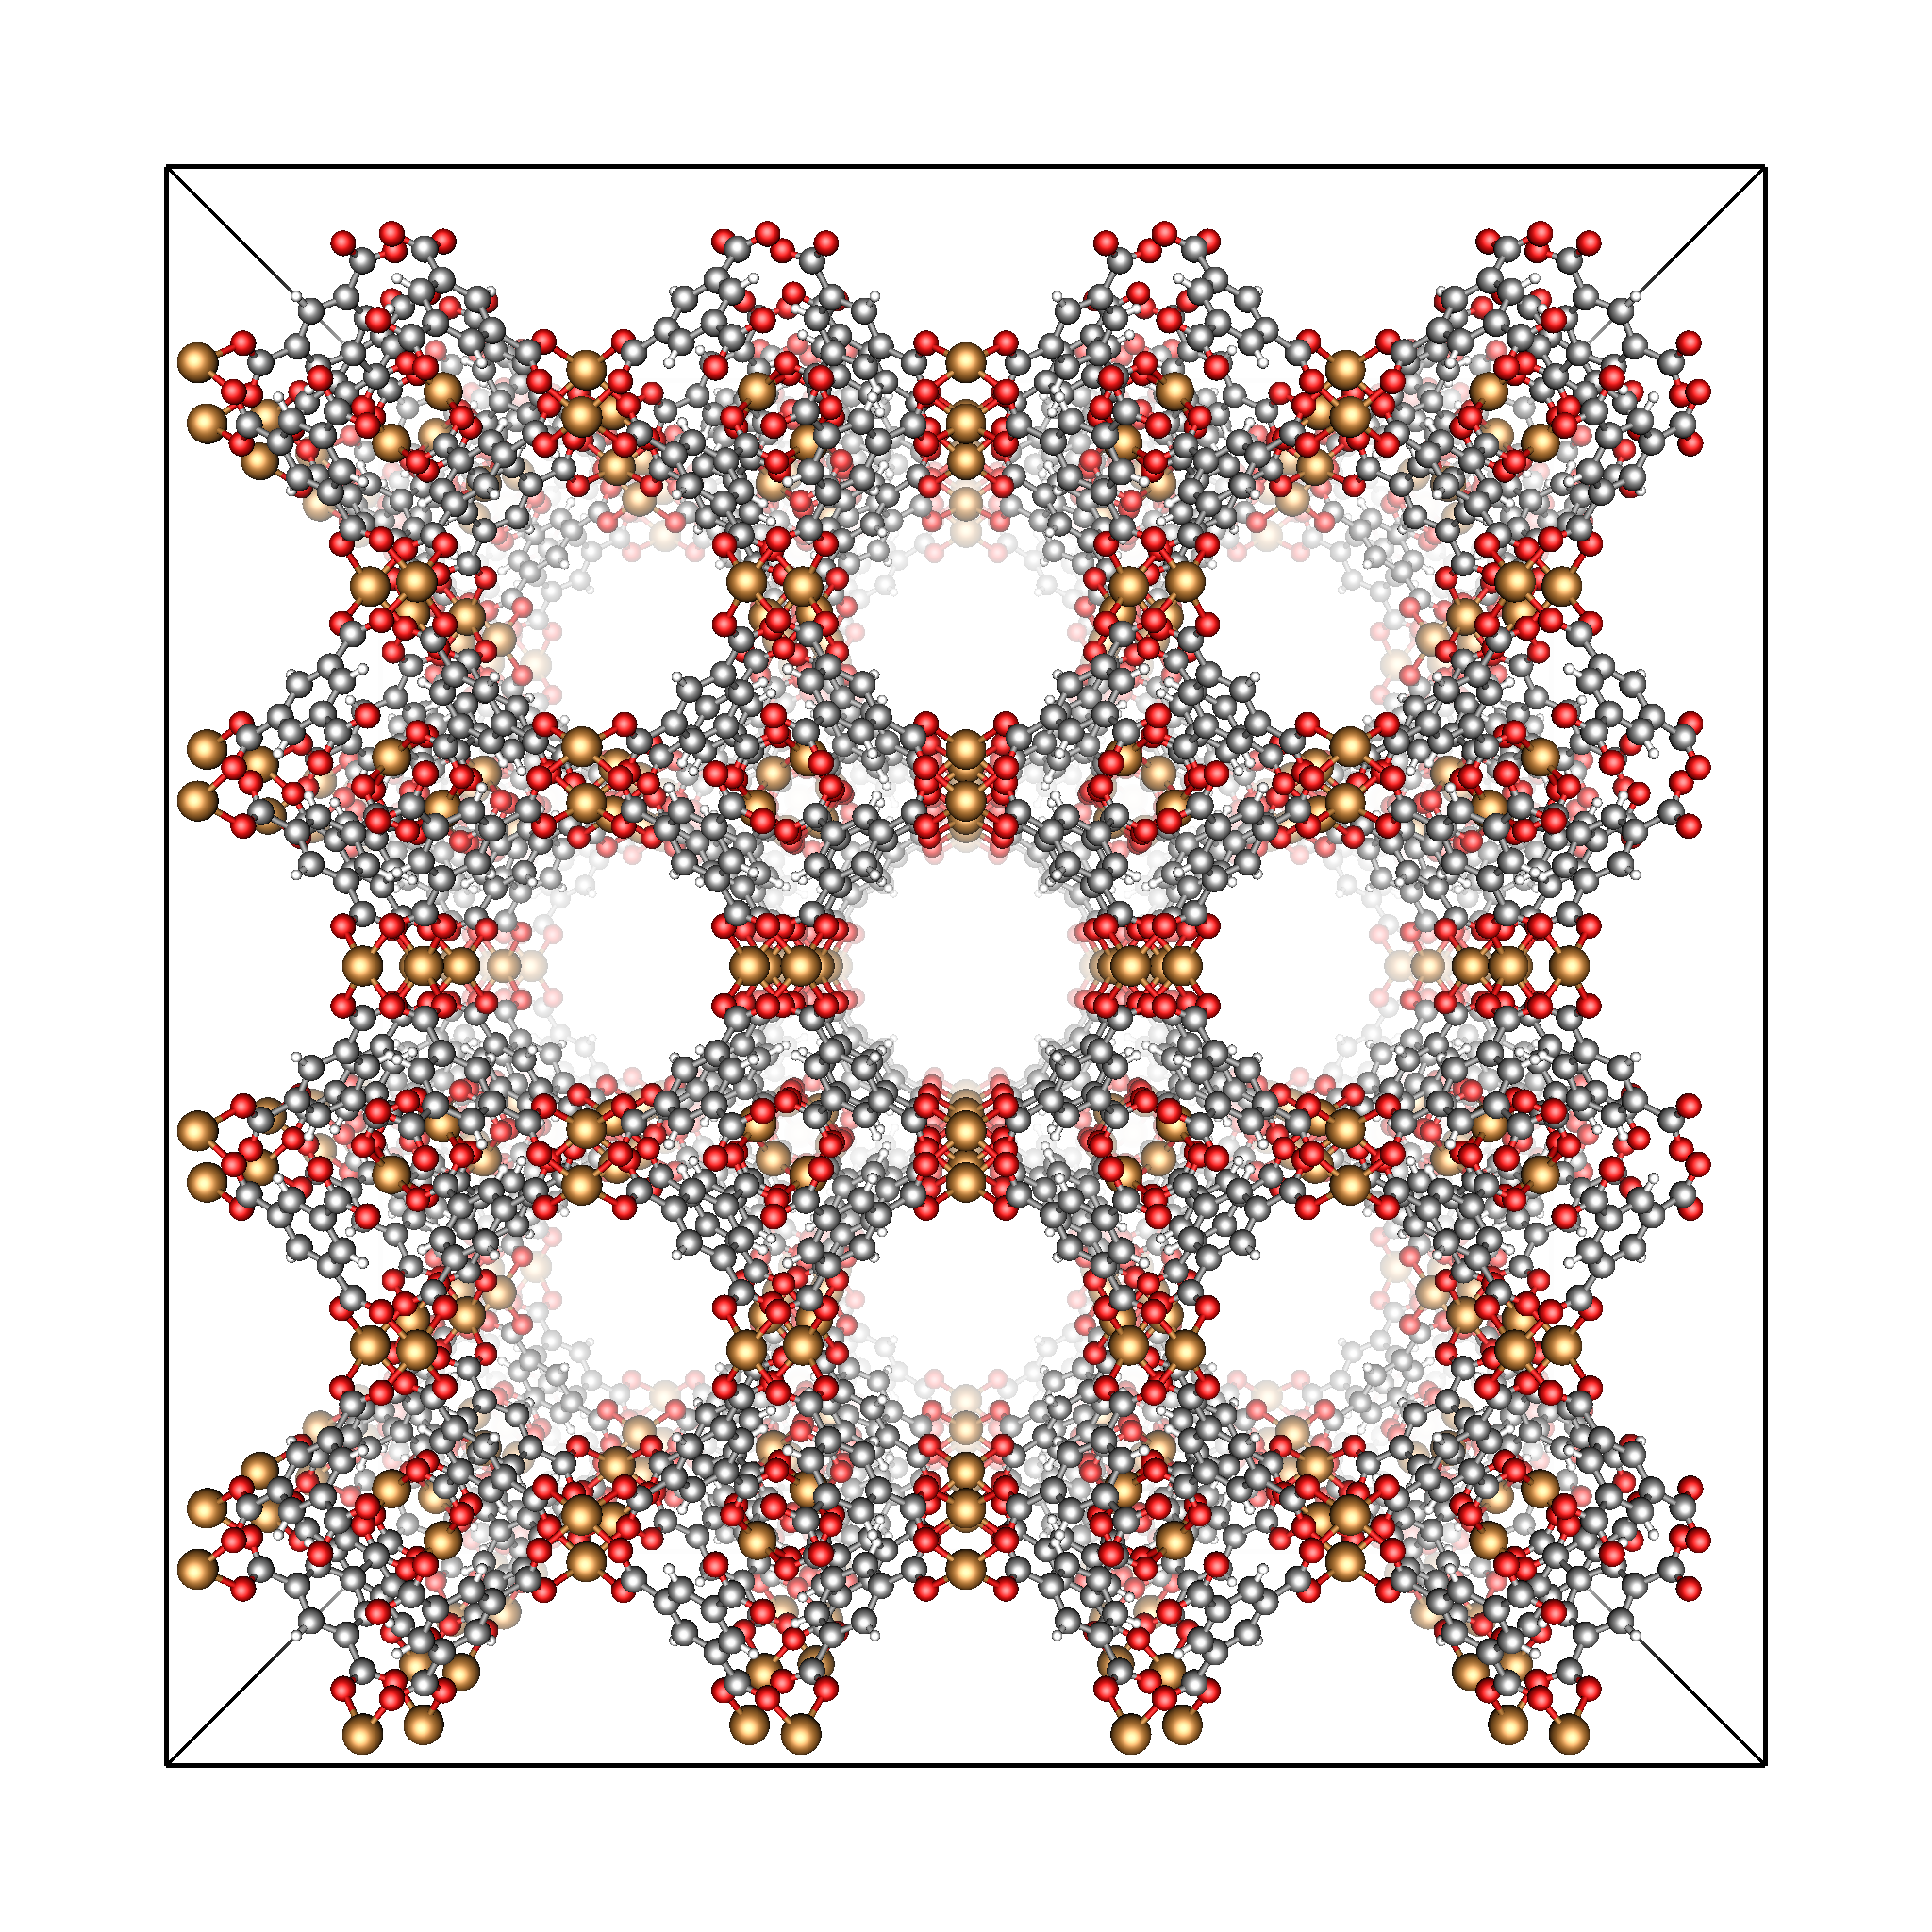
\includegraphics[width=0.6\columnwidth]{hkust-1_fancy.png} \label{fig:example_MOF}
    }
    \qquad
    \subfloat[][]{
        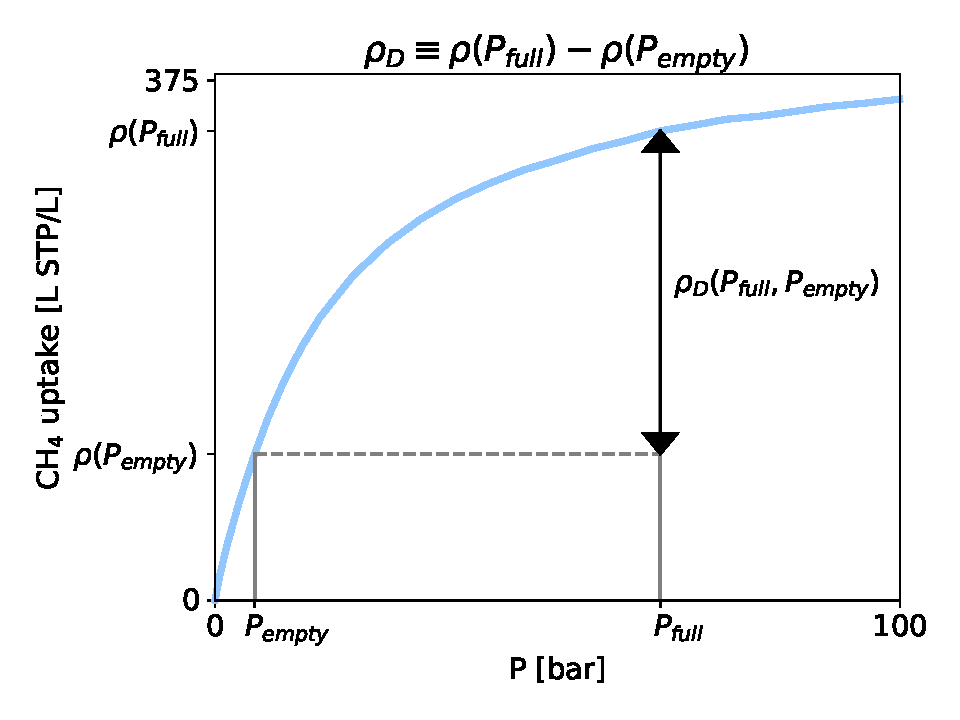
\includegraphics[width=0.98\columnwidth]{usable_capacity_illustration_toy_ish.pdf} \label{fig:delcap}
    }
    \caption{Gas storage and delivery using metal-organic frameworks (MOFs). (a) the crystal structure of an archetype MOF, CuBTC \cite{chui1999chemically}. (b) the methane adsorption isotherm in CuBTC \cite{chui1999chemically} at 298 K (blue) (data from Ref.~\cite{mason2014evaluating}). The deliverable capacity $\rho_D$ is illustrated as the density of gas in the MOF at the storage pressure $\pfull$ minus the density at the discharge pressure $\pempty$.
    }
    \label{fig:fig1}
\end{figure}

To set realistic performance targets and optimally allocate resources for research efforts, in this work, we present a theoretical framework that places an intrinsic upper limit on the deliverable capacity of gas in a rigid porous material and uses as input the experimentally measured properties of the bulk gas. Our extremum is provided by a substrate that offers a spatially uniform potential energy field felt by the gas. Applying our framework to methane and hydrogen gas, we find the US DOE deliverable capacity targets for natural gas and hydrogen storage and delivery are theoretically possible, but sufficiently close to the upper bound as to be impractical for any real porous material. Optimistically, new paradigms outside the scope of applicability of our theoretical framework, such as gas-induced structural transitions of the material, hold promise for meeting these targets, as evidenced by flexible MOF Co(bdp) which currently boasts the largest methane deliverable capacity~\cite{mason2015methane}.

% Jordan: I commented this out!
% To optimally allocate resources for research efforts and set realistic performance targets, it is important to assess the thermodynamic limits of technologies. Here, we present a theoretical framework that places an intrinsic upper limit on the deliverable capacity of gas in a nanoporous material and uses as input experimental measurements of the bulk gas. Applying our framework to methane and hydrogen gas, we find the DOE deliverable capacity targets for natural gas and hydrogen storage and delivery are theoretically possible, but sufficiently close to the upper bound as to be impractical for any real porous material.

\section{Gas storage \& delivery by isothermal, pressure-swing adsorption}
% Here, we pose the context and question that we address in this work.
% Consider pure gas storage and delivery by isothermal, pressure-swing adsorption \cite{sircar2002pressure}.
Consider a pressure vessel onboard a vehicle (i.e. fuel tank) packed with porous material. At the filling stage, the tank is connected to a (pure) gaseous reservoir at pressure $\pfull$ and allowed to equilibrate. At this point, the adsorbed gas tank is considered full. While driving, gas desorbs from the adsorbent to the engine/fuel cell, driven by a pressure differential.
The tank is considered depleted/empty when the pressure has dropped to $\pempty$, the pressure at which the flow rate of gas from the tank to the engine is insufficient.
%
However, given $\pempty \neq 0$ (pulling vacuum), residual gas will remain trapped in the adsorbent. Therefore, the driving range of the vehicle is primarily determined by the \emph{deliverable capacity}, defined as the density of gas in the tank at $\pfull$ minus density of the the residual gas remaining at $\pempty$. The [isothermal, volumetric] deliverable capacity is an intrinsic property of the nanoporous material and its interaction with the gas.
%Precisely, let $\rho(p; T)$ be the density of gas in the adsorbent when in equilibrium with a bath of pure gas at pressure $p$ and temperature $T$, the \emph{adsorption isotherm}; $\rho(p,T)$ is essentially the equation of state of the gas adsorbed in the porous material. The [intrinsic, isothermal] deliverable capacity $\rho_D$ of the gas in the adsorbent is:
%\begin{equation}
%    \rho_D(\pfull, \pempty; T) \equiv \rho(\pfull; T) - \rho(\pempty; T).
%    \label{eq:delcap}
%\end{equation}
% The pressures $\pfull$ and $\pempty$ correspond to chemical potentials $\mufull$ and $\muempty$ via an equation of state for the gas.
% Eqn.~\ref{eq:delcap}
% This assumes that the tank reaches equilibrium %, neglecting the kinetics of ad/desorption
% at the end of the filling and depletion stages. 

%The assumption of isothermal operation neglects (i) heat released/consumed during ad/desorption, which can diminish the deliverable capacity by raising/lowering the temperature of the adsorbent during filling/discharge \cite{mota1997dynamics,chang1996behavior}, and (ii) an engineering strategy to use waste heat from the engine to heat the adsorbent and drive off residual gas when it nears $\pempty$ \cite{gomez2014exploring}. 

%Second, an engineering strategy to increase the deliverable capacity beyond the isothermal deliverable capacity is to reroute waste heat from the engine to the adsorbed gas tank during delivery. By raising the temperature of the adsorbent during the discharge stage, we drive off a fraction of the residual gas that would otherwise remain when the tank reaches $\pempty$ . In such a case, the [non-isothermal] deliverable capacity of the tank is $\rho(\pfull, T)-\rho(\pempty; T_H)$ where $T_H$ is the temperature to which we heat the adsorbent at discharge. This strategy, however, requires a more complicated design.

% \begin{limitation}\label{limit:isothermal}
% We assume isothermal pressure-swing adsorption. It is possible to achieve a greater deliverable capacity by raising the temperature of the adsorbent as the gas is extracted to drive off the residual gas.
% \end{limitation}

\section{Review of previous work}
There has been considerable work attempting to establish an upper bound on the isothermal deliverable capacity in pressure-swing adsorption.
% We now review previous work towards placing an upper bound on the isothermal deliverable capacity of hydrogen or methane by pressure-swing adsorption.
% The first body of work rests on the simplified Langmuir model; the second body of work rests upon imposing energetic models for the gas-substrate and gas-gas interactions.

Early work showed that, in the simplified Langmuir model, there exists an optimal free energy of adsorption (which determines the Langmuir constant) that maximizes the deliverable capacity $\rho_D$~\cite{matranga1992storage,bhatia2006optimum,simon2014optimizing}.
If the gas-substrate interaction is too weak (strong), too little (much) gas adsorbs (is retained) at $\pfull$ ($\pempty$), diminishing $\rho_D$. An upper bound on the deliverable capacity of a Langmuir material follows if each adsorption site is endowed with the optimal free energy of adsorption. However, remaining is the question of how many adsorption sites per volume a porous material can practically offer, under the constraint that these adsorption sites offer the optimal free energy of adsorption. Moreover, gas-gas attractions, neglected in the Langmuir model, could recruit more gas in the material at $\pfull$ than at $\pempty$ and enhance the deliverable capacity~\cite{simon2014optimizing}.

G\'omez-Gualdr\'on \emph{et al.}~\cite{gomez2017impact} introduced a model that accounted for gas-gas interactions via an intermolecular potential and idealized the substrate in two different ways: (1) discrete adsorption sites packed into an FCC lattice and (2) a volume endowed with a spatially uniform, background potential energy field. According to molecular simulation of methane adsorption, the ARPA-E deliverable capacity target of 315 L STP/L could be reached in both of these idealized substrates.
%The ARPA-E target of 315 L STP/L was reached when adsorption sites were endowed with an optimal heat of adsorption of 11.5 kJ/mol and adsorption sites were $5.3$ \AA~apart. In a second model, they endowed a volume with a background potential energy field, then simulated the adsorption of methane in the volume in the grand-canonical ensemble, using a Lennard-Jones potential for methane-methane interactions. The maximal deliverable capacity of 357 L STP/L was achieved with a background heat of adsorption of 8.6 kJ/mol. 
However, both models neglected the space occupied by atoms of the porous material that are needed to endow the adsorption sites/volume with the attractive potential energy. % To address this, in the third model, they constructed pseudo materials by placing Lennard-Jones spheres in space with tunable well depths. When constrained to form a connected network, none of the psuedo-materials reached the ARPA-E deliverable capacity target.

A third body of work attempted to account for both gas-gas interactions \emph{and} steric interactions of the gas with the atoms of the porous material.
% explores the upper limits of the deliverable capacity while accounting for gas-gas interactions \emph{and} the atoms of the porous material that are required to attract the guest; these material atoms exclude the adsorbate from regions of the control volume. 
%More works obtained an empirical upper bound on the deliverable capacity by explicitly accounting for the atoms of the material needed to create the potential energy field felt by the gas molecules.
Simulations of methane adsorption in hundreds of thousands of explicit nanoporous crystal structures---both real and hypothetical---suggested that the ARPA-E deliverable capacity target is infeasible~\cite{simon2015materials}; the highest simulated methane deliverable capacity was 196 cm$^3$~STP/cm$^3$. Confidence in this conclusion rests upon (i) the accuracy of the intermolecular potentials describing the molecular interactions and (ii) the sufficient sampling of material space, i.e.\ that the structures considered are representative of the set of possible materials. To further explore material space and address sensitivity to the potentials used, scaling the Lennard-Jones potential well depths of material atoms to model enhanced interactions~\cite{gomez2014exploring}, placing Lennard-Jones spheres in a unit cell randomly to form ``pseudo-materials''~\cite{kaija2018high}, and generating fictitious potential energy fields via a generative adversarial network trained on zeolite structures~\cite{lee2019predicting} all generated model substrates that all failed to meet the ARPA-E methane deliverable capacity target.

% Brown and Freeman \cite{bhown2011analysis}

In this work, we place a rigorous upper bound on the deliverable capacity of a pure gas in a rigid substrate by endowing a control volume with a spatially uniform background energy field. Instead of using a molecular model for the gas~\cite{gomez2017impact}, we use the experimental equation of state to account for gas-gas interactions. In addition, we prove using the calculus of variations that this spatially uniform substrate yields a maximal deliverable capacity. We use our framework to place an upper bound on the deliverable capacity of methane and hydrogen.

\section{An upper bound on the deliverable capacity of a pure gas in a rigid porous material}\label{sec:upper-bound}
\begin{figure}
  \centering
  \includegraphics[width=\columnwidth]{methane-298-rho-mu}
  \caption{The density of bulk methane, the ideal gas, and adsorbed gas in several MOFs at 298\ K as a function of chemical potential (bottom axis) and pressure (top axis). The bulk methane density is from the National Institute of Standards and Technology (NIST)~\cite{nist}. The methane adsorption isotherms in the MOFs are experimental data from Ref.~\cite{mason2014evaluating, furukawa2009storage}.
  }
  \label{fig:density-vs-mu-ch4}
\end{figure}

We now develop a thermodynamic framework that places an upper bound on the deliverable capacity of any pure gas in a rigid porous material.

The thermodynamic properties of a bulk, pure gas are characterized by an equation of state. 
Of particular interest for gas storage and delivery is the density of the gas as a function of chemical potential $\mu$ and temperature $T$, $\rho_g(\mu,T)$, which is shown for methane gas in Fig.~\ref{fig:density-vs-mu-ch4} at $T=298$\ K. For comparison, we also show the density of methane adsorbed into several porous materials.

% \davidsays{This paragraph could move considerably later. Or cut entirely?}
% We model the interaction of substrate with gas as a simple Gibbs free energy of adsorption per mole (or atom) \gst.  We will assume that this Gibbs free energy is independent of the concentration of gas.  At low concentrations, this assumption is reasonable, because the gas molecules can be assumed to be widely separated and their interactions weak.  In the limit of high concentrations, we expect that the attraction of the gas to the substrate will be diminished, since the ``good spots'' will already be occupied.  The choice of a concentration-independent $\gst$ will thus have a tendency to overestimate the deliverable capacity, providing an upper bound (for more on this, see Sec.~\ref{sec:qualitative-max}).

To place an upper bound on the deliverable capacity, consider a substrate whose sole interaction with the gas is to introduce a spatially uniform potential energy $\V$
for gas molecules in the control volume (where $\V<0$ for an attractive potential). Because this interaction is uniform within the substrate, the gas-gas interactions and thus fluid structure in such a substrate are identical to those of the pure gas at the same density and temperature. This allows us to obtain the adsorption properties of this model substrate using the experimentally measured properties of the pure gas~\cite{nist}. 
Intuitively, the deliverable capacity of a gas in such a homogeneous substrate with the optimal potential energy is an upper bound because, in a realistic material, (i) spatial inhomogeneity of the potential energy results in some points in the control volume offering a suboptimal attraction for the gas and (ii) the atoms required to create the potential field will exclude gas from occupying a fraction of the control volume.
%\corysays{the suboptimal energy is hard to argue since that would affect entropy too...}

% \corysays{I propose to replace ``homogenous'' with ``spatially uniform'' everywhere instead of using both interchangeably.
% \davidsays{We replaced ``homogeneous potential'' with spatially uniform, but were less confident replacing ``homogeneous substrate'', which has a slightly different meaning, and might need a slightly different name.  e.g. maybe ``uniform substrate'' or ``model substrate''?}}

%\corysays{what do u think about callin this an ``ideal substrate'' or giving it some name so we can refer to it hereon? \davidsays{I think I'd prefer ``homogeneous substrate'' or ``idealized substrate''}}

%\subsection{Finding the density}\label{sec:finding-n}

The spatially uniform potential $\V$ representing gas-substrate interactions behaves as an external potential and effectively shifts the chemical potential (or, equivalently, molar Gibbs free energy) of the gas in the material, just as gravitational potential energy causes the density of air to vary with altitude.  Consequently, the density of gas in our homogeneous substrate is:
\begin{align}
    \rho(\mu,T) &= \rho_g(\mu - \V,T). \label{eq:mof-density}
\end{align}
See Sec.~\ref{sec:V_shifts_chem_pot} for a derivation.
% where $\rho_g(\mu,T)$ is the density of the pure gas at chemical potential $\mu$, shown for methane in Fig.~\ref{fig:density-vs-mu-ch4}. 
% cory says: ^ we already defined \rho_g in pargraph above.

The deliverable capacity of gas in our homogeneous substrate is thus:
\begin{align}
    \rho_D(\V,T) &= \rho(\mufull,T) - \rho(\muempty,T),
    \label{eq:DofPhi}
    \\
    &= \rho_g(\mufull-\V,T) - \rho_g(\muempty-\V,T),
\end{align}
where $\mufull$ and $\muempty$ are the chemical potentials corresponding to the pressures $\pfull$ and $\pempty$, respectively.
Thus, $\rho_D$ for our homogeneous substrate as a function of $\V$ is the difference between two shifted versions of $\rho_g(\mu; T)$.
Figure~\ref{fig:methane-298-D} shows the two shifted bulk methane density curves and their difference.
The horizontal axis
is the difference in molar Gibbs free energy at fixed density and temperature between the gas within the substrate and the pure gas (\gst), which is equal to $\V$ in our model.
We see a potential $\V$ that maximizes the deliverable capacity of our ideal substrate, balancing the need to maximize the density at $\pfull$ against the need to minimize residual gas retained at $\pempty$. 
%Our theoretical framework thus recovers an upper bound on the deliverable capacity of methane (298\ K, $\pfull=$65\ bar, $\pempty=$5.8\ bar) in porous materials as 374\ L STP/L.
The optimal deliverable capacity of methane (298\ K, $\pfull=$ 65\ bar, $\pempty=$ 5.8\ bar) in our ideal, spatially uniform substrate is 374\ L STP/L, \red{achieved for $\V_{opt} = ...$}.
%
%As a ballpark, we can expect the attractive potential to be optimal around the maximum slope of $\rho_g(\mu)$.  This is the point where the steric repulsion between the gas atoms starts leading to saturation of the density.

An essential question is whether our idealized substrate offering the spatially uniform potential $\V_{opt}$ for the gas places an upper bound on the deliverable capacity in all rigid porous materials. 
%yields the maximum deliverable capacity over all possible potential energy fields. 
In the SI (see Section~\ref{sec:fixme} \davidsays{Look up section label}), we show that our idealized substrate with spatially uniform potential $\V_{opt}$ yields an \emph{extremum} of the deliverable capacity over all possible \emph{static potential energy fields}, provided the gas does not crystallize at the temperature and in the density range of interest. The potential energy field is \emph{static} if it is unaffected by the presence of the gas; consequently, our model does not apply to flexible materials that undergo gas-induced conformation changes \cite{schneemann2014flexible}. We next argue that this extremum is a maximum by addressing two alternative possibilities: the extremum could turn out to be (i) a saddle point or (ii) a local, rather than global, maximum.

Fig.~\ref{fig:methane-298-D} clearly shows that $\V_{opt}$ provides a maximum $\rho_D$ over all \emph{spatially uniform}, static potential energy fields. To qualitatively argue that the spatially uniform potential $\V_{opt}$ provides a maximum deliverable capacity over \emph{all} (including non-spatially uniform) static potential energy fields (a broader claim), consider a non-spatially-uniform variation on $\V_{opt}$.
We will show that the effect of this variation is to reduce the deliverable capacity.
At low adsorbed gas densities, the lowest-energy positions will be preferentially occupied, while at higher densities, the additional gas molecules will be forced into higher energy locations. Thus, the mean attraction will be lowest at \pfull\  and highest at \pempty.  This will result in $\gst$ increasing monotonically with with pressure.  As shown in the Supplementary Information (see Sec.~\ref{sec:monotonic}), this results in the deliverable capacity of a non-uniform potential being lower than the deliverable capacity of a uniform potential with $\V=\gst$ for either $\pfull$ or $\pempty$.
Thus a spatially uniform potential will give the best deliverable capacity amongst all static potential energy fields that give the same $\gst$, and the \emph{optimal} uniform potential $\V_{opt}$ will give the a greater deliverable than any static non-uniform potential.

% Yo David, I changed ur paragraph below. tell me wut u think.
% To qualitatively argue that the spatially uniform potential $\V_{opt}$ provides a \emph{maximum} deliverable capacity over all static potential energy fields, consider the case of a material that offers a non-spatially-uniform potential energy felt by the gas molecules.We wish to show that this material will have a lower deliverable capacity than our ideal substrate. At low adsorbed gas densities, the lowest-energy positions will be preferentially occupied, while at higher densities, some of the gas molecules will be forced into higher energy locations. Thus, the mean attraction will be lowest when the tank is ``full,'' and highest when the tank is ``empty.'' This is the opposite of what we would want to achieve a high deliverable capacity. Based on this qualitative reasoning, we expect the spatially uniform potential \red{$\V_{opt}$} to give the maximal deliverable capacity, since it will provide the most attraction for the molecules added at high densities.

% \corysays{``To qualitatively argue that the spatially uniform potential provides a \emph{maximum} deliverable capacity'' do we need to qualify that this spatially uniform potential must hv the optimal $\V$? obviously a spatially uniform potential can be better than a spatially uniform one with a poor $\V$. maybe we should start with our optimal homogenous potential, then say introduce a little blip in it from there, like in calculus of variations.}

\begin{figure}
    \centering
    \includegraphics[width=0.95\columnwidth]{methane-298-n-vs-G}
    \caption{The deliverable capacity of methane as a function of the attractive Gibbs free energy $|\gst|$.
    Experimental deliverable capacities for several MOFs (data from Ref.~\cite{mason2014evaluating, furukawa2009storage}) are shown along with the experimental values for $\gst$ at the empty and full pressures shown as dots connected by a line (not visible at this scale).}
    \label{fig:methane-298-D}
\end{figure}

\section{Results}
Although our theoretical framework allows us to place an upper bound on the deliverable capacity of many different gases in a rigid porous material, we focus on the maximal deliverable capacity of methane and hydrogen gas in our homogeneous substrate due to their application as transportation fuels. To characterize the density of the gases, $\rho_g(p, T)$, we use experimental data from NIST~\cite{nist}, which naturally includes quantum effects that particularly affect hydrogen at low temperature~\cite{kumar2006quantum}. In the context of storage onboard passenger vehicles, we compare our upper bound with several prominent porous materials using experimental adsorption isotherms from the literature; we also compare with deliverable capacity targets set by the US DOE.

Figure~\ref{fig:methane-298-D} shows the upper bound for methane storage at room temperature~(374~cm$^3$~STP/cm$^3$). In addition to the predicted maximum deliverable capacity as a function of \gst,
\corysays{subtlety here: isnt ur proof restricted to saying $\V_{opt}$ provides the upper bound? does it really prove that, for fixed and nonoptimal $\gst$, a spatially uniform potential is optimal over a non-spatially uniform one? I don't think it does...}
the ARPA-E target of 315~cm$^3$~STP/cm$^3$~\cite{arpaemove} is shown for context. For an adsorbent with at least 84\% void fraction, the ARPA-E target is theoretically possible. The experimental deliverable capacities of several adsorbents~\cite{mason2014evaluating} are also shown over a range of $\gst$ (converted from the measured adsorption isotherm as explained in \davidsays{confirm this} Sec.~\ref{sec:phi-is-delta-g}). These can be compared with the highest observed deliverable capacities for methane at room temperature in rigid materials, up to 208~cm$^3$~STP/cm$^3$~\cite{simon2015materials}. 
% don't think the below is helpful or correct: Gst opt is reached by some... there are void fraction constraints too.
% To reach the ARPA-E target, an adsorbent material with a higher $|\gst|$ would need to be found. 

\corysays{I know it doesn't matter, but should we choose L STP/L or cm3 STP/cm3? we use both, some might get confused/distracted? \davidsays{We chose to use the units used for each of the targets thinking it would be more familiar and/or easier to compare.  I don't like either set of units, and if we were to pick ``our'' choice, I'd lean towards something dimensionless with a sane comparison (e.g. relative to the gas density at our high pressure)}}

\corysays{need to explain why the MOFs are lines not points... that \gst has a range for MOFs.
\jpsays{due to a different deliverable capacity at full pressure and empty pressure. For hydrogen the SI (by Paula Garcia-Holley) has total uptake plots so we could make a curve even but would have a lot of error due to manual extraction?}}

\begin{figure}
    \centering
    \includegraphics[width=0.95\columnwidth]{hydrogen-298-n-vs-G}
    \caption{Deliverable capacity of hydrogen at room temperature as a function of the attractive Gibbs free energy $|\gst|$.  Experimental deliverable capacities for several MOFs are shown along with the experimental values for $\gst$ at the empty and full pressures shown as x's connected by a line.}
    \label{fig:hydrogen-298-D}
\end{figure}

\corysays{Figs.~\ref{fig:hydrogen-298-D} ~\ref{fig:methane-298-D} why not just let $\gst$ be negative and have an arrow pointing in direction of more attraction? as written the legend is not correct since those are not the functions being shown. in the main text we never discussed what \gst is for the MOF and why the MOFs are lines not points (\gst is a function of density now)}

\jpsays{I edited everything below this comment. The original is commented out}

Storage of hydrogen is considerably more challenging owing to its relatively weak interaction with adsorbents. The DOE ULTIMATE deliverable capacity target~\cite{DOE} is within 6\% of the upper bound at 25$^\circ$C \red{check}. Figure~\ref{fig:hydrogen-298-D} shows the theoretical upper bound curve for hydrogen storage along with a range of experimental measurements for known MOFs.  The DOE ULTIMATE deliverable capacity target is theoretically possible, however by such a small margin that we can safely rule out the possibility of reaching this target through storage and delivery of hydrogen in \emph{any} rigid substrate at room temperature. Such a material would require a void fraction of at least 94\% \red{check}. On top of this, the DOE ULTIMATE target requires an optimal $|\gst|$ of 10~kJ/mol which is far greater than what is found in observed porous materials. This reflects the known fact that hydrogen interacts with substrates far more weakly than methane does. One possibility that has been pursued is storage at cryogenic temperatures. See Section~\ref{sec:cryo-hydrogen} in the Supplementary Information for the upper bound for storage of hydrogen at 77 K.

Why do we not experimentally observe materials approaching the upper bound on the deliverable capacity? Foremost, any adsorbent substrate will be composed of atoms, which will exclude the gas from some volume. Due to strong short-range interactions, substrate atoms must be uniformly distributed to achieve strong attraction for gas atoms. Uniform atom distribution sets a limit on the pore volume.
% Because strong interactions are short-range, achieving a strong attraction requires that substrate atoms be distributed throughout the volume, which places a limit on the pore volume.
In contrast, real materials have a spatially non-uniform attraction for gas atoms. The result of this is that there are regions of space with non-optimal attraction. For hydrogen, there is the further issue that there are \emph{no} known physical interactions that are sufficiently strong to give an optimal deliverable capacity at room temperature.
% Finally, real materials must have a spatially non-uniform attraction for gas atoms, resulting in some regions of space where the attraction is not optimal. For hydrogen, there is the further issue that there are \emph{no} known physical interactions that are sufficiently strong to give an optimal deliverable capacity at room temperature.

\section{Conclusion}
We have established an upper bound on the deliverable capacity via pressure-swing adsorption in rigid porous solids based on experimentally measured properties of pure gases. While these upper bounds do not rule out the discovery of materials that reach current DOE targets, they cast strong doubt on the possibility of achieving these goals when we consider the additional constraints imposed due to steric hindrance between substrate atoms and the adsorbate. Our upper bound does indicate that those goals cannot be exceeded by more than 19\% for methane and 6\% for hydrogen \red{check}. Fortunately, there are some limitations to these upper bounds which suggest avenues for future developments which could allow the targets to be met.

The first limitation of our proof is that we restricted ourselves to \emph{isothermal} pressure swing storage. By raising the temperature of the adsorbent during gas discharge to drive off residual gas~\cite{gomez2014exploring}, the deliverable capacity could be enhanced, albeit at the cost of a more complicated engineering design of the fuel tank and vehicle.
%While this approach poses engineering challenges, in principle it could allow an arbitrarily large deliverable capacity.

% \corysays{no, cant lower filling temp. when park it will heat up then go above pressure rating of tank...}

The second limitation of our proof arises in the assumption of a rigid substrate. The rigid substrate acts as a static potential energy field for gas molecules that is unchanged by the adsorption of gas.
% The second limitation of our proof arises in the assumption of a rigid substrate, which acts as a static potential energy field for gas molecules that is unchanged by the adsorption of gas.
For most porous materials this is a reasonable approximation, and this assumption is frequently made in both the simulation and theory of porous materials~\cite{witman2017influence}. However, there are cases where the substrate can in effect provide a very strongly gas-density-dependent interaction through structural flexibility~\cite{schneemann2014flexible}. A flagship example is MOF Co(bdp)~\cite{choi2008broadly}, which possesses a wine-rack-like topology capable of hinge motion. At low methane pressure, Co(bdp) adopts a collapsed, nonporous state, but expands to a porous state and fills with gas at higher pressures~\cite{mason2015methane}. This allows Co(bdp) to fully expel its residual gas at low pressures.
Our upper bound does not consider such material effects and thus flexible materials could have significantly higher deliverable capacities.
% Such materials can indeed violate our upper bound and thus could lead to significantly improved deliverable capacities.

We note that our upper bound can readily be applied to the storage of other gasses of interest, with the proviso that the gas is far from crystallization. Our code is available at \davidsays{XXXXX}.

% \clearpage


% Here we will articulate the assumptions required for our upper bound to hold. Some of these assumptions serve as a guide for chemists who aim to synthesize a material that violates our upper bound.

% Our proof that the spatially uniform potential is an extremum assumes that the fluid is stable at the temperature and densities involved.
% \begin{limitation}\label{limit:crystallization}
% Our proof assumes the gas is cannot become spontaneously solid at the temperature of interest.
% \end{limitation}
% Our upper bound will \emph{not} be valid for gasses which may crystallize in their pure form. This is because a periodic potential can interact with a high-density crystal far more strongly than it interacts with a low-density gas.  We are not aware of a practical application of this principle, but theoretically it is possible.  For the application of gas storage for light gasses such as methane or hydrogen at moderately high temperatures (say liquid nitrogen or warmer), the pure gas is sufficiently far from its crystal form that we need not concern ourselves with crystallization.  We do not see this particular assumption as one that can be worked around.

% There remains the possibility that the spatially uniform potential is a local maximum, but there is another global maximum.  We do not see how to formally rule out this possibility for an arbitrary gas-gas interaction, but the qualitative arguments above seem sufficient to rule out this possibility for a real gas.

% However, there was a more fundamental assumption, which is that the porous material acts as an effective potential for the gas molecules, and that the gas-gas interaction is unmodified.
% \begin{limitation}\label{limit:field}
% Our proof assumes the interaction of the gas with the substrate does not modify the substrate.  Equivalently,  the interaction of substrate with gas operates as a simple potential energy field.
% \end{limitation}
% For \emph{most} porous materials this seems likely to be a pretty good approximation.  However, there are unusual cases where the substrate can in effect provide a very strongly density-dependent interaction.  This is perhaps easiest to see in the example of \davidsays{look up the collapsing MOFs description from the RMS-MOF paper}, in which the gas can introduce a phase change in the solid, which has the effect of drastically lowering the density of gas in the material.  Such materials can indeed violate our upper bound. \davidsays{Remember to discuss this in the conclusions or perhaps discussion, we can frame these limitations as guides.  The limitations of our upper bound are the design requirements for a material that will do any better.}


% [impurities?]

% \section{Conclusion}
% As many have suspected \davidsays{cite previous work}, pressure-swing adsorption in rigid porous solids is not going to enable reaching targets.  \davidsays{conclude explicitly about each target}  Unlike previous work, our upper bound on deliverable capacity is based on experimentally known properties of the gas of interest rather than simulations.

% The limitations on our proof of an upper bound on the deliverable capacity provide hints as to approaches that could in principle achieve the targets.  In this paper we have identified three limitations of our upper bound on the deliverable capacity.  Two of these three limitations suggest engineering strategies that do hold promise of achieving the targets for hydrogen and methane storage.  Limitation \ref{limit:crystallization}, which states that the gas must not crystallize does not means for improvement, since it is a limit on the gasses to which our bound may be applied, and neither hydrogen nor methane are in any danger of crystallizing.

% Crystal density vs. pelletiziation density.

% A more subtle limitation of our proof is that it assumes that the substrate itself is not modified by the presence of the gas.  While this assumption is never precisely true, since any adsorbed atom will change the electron distribution of the substrate to some degree, it tends to be sufficiently accurate that most atomistic simulations can get away with assuming that the substrate is unmodified.  A dramatic exception to that rule is the field of flexible MOFs, in which the presence of the gas can induce a phase change which can \emph{drastically} modify the gas-substrate interaction~\davidsays{cite experiments}\cite{witman2019}.


% wut about mixtures?